\pdftrailerid{}
\documentclass[11pt]{article}
\usepackage[T1]{fontenc}
\usepackage{lmodern}
\ifdefined\pdfglyphtounicode
  \pdfgentounicode=1
  \pdfglyphtounicode{tfm:lmex10/parenleftbig}{0028}
  \pdfglyphtounicode{tfm:lmex10/parenrightbig}{0029}
  \pdfglyphtounicode{tfm:lmex10/vextendsingle}{23D0}
  \pdfglyphtounicode{tfm:lmex10/parenleftBig}{0028}
  \pdfglyphtounicode{tfm:lmex10/parenrightBig}{0029}
  \pdfglyphtounicode{tfm:lmex10/parenleftbigg}{0028}
  \pdfglyphtounicode{tfm:lmex10/parenrightbigg}{0029}
  \pdfglyphtounicode{tfm:lmex10/floorleftbigg}{230A}
  \pdfglyphtounicode{tfm:lmex10/floorrightbigg}{230B}
  \pdfglyphtounicode{tfm:lmex10/braceleftbigg}{007B}
  \pdfglyphtounicode{tfm:lmex10/bracerightbigg}{007D}
  \pdfglyphtounicode{tfm:lmex10/parenleftBigg}{0028}
  \pdfglyphtounicode{tfm:lmex10/parenrightBigg}{0029}
  \pdfglyphtounicode{tfm:lmex10/braceleftBigg}{007B}
  \pdfglyphtounicode{tfm:lmex10/parenlefttp}{239B}
  \pdfglyphtounicode{tfm:lmex10/parenrighttp}{239E}
  \pdfglyphtounicode{tfm:lmex10/parenleftbt}{239D}
  \pdfglyphtounicode{tfm:lmex10/parenrightbt}{23A0}
  \pdfglyphtounicode{tfm:lmex10/summationtext}{2211}
  \pdfglyphtounicode{tfm:lmex10/producttext}{220F}
  \pdfglyphtounicode{tfm:lmex10/summationdisplay}{2211}
  \pdfglyphtounicode{tfm:lmex10/productdisplay}{220F}
  \pdfglyphtounicode{tfm:lmex10/integraldisplay}{222B}
  \pdfglyphtounicode{tfm:lmex10/intersectiondisplay}{22C2}
  \pdfglyphtounicode{tfm:lmex10/tildewide}{02DC}
  \pdfglyphtounicode{tfm:lmex10/bracketleftBig}{005B}
  \pdfglyphtounicode{tfm:lmex10/bracketrightBig}{005D}
  \pdfglyphtounicode{tfm:lmex10/radicalbigg}{221A}
  \pdfglyphtounicode{tfm:lmsy10/mapsto}{007C}
\fi
\usepackage[margin=1.05in]{geometry}
\usepackage{amsmath,amssymb,amsthm,mathtools}
\usepackage{microtype}
\usepackage{enumitem}
\usepackage{flafter}
\usepackage{tikz}
\usetikzlibrary{arrows.meta,positioning}
\usepackage{xcolor}
\usepackage[colorlinks=true,linkcolor=blue!45!black,citecolor=blue!45!black,
  urlcolor=blue!45!black,pdfauthor={OpenAI},
  pdftitle={A single-lattice covering bound of order n log n}]{hyperref}
\newtheorem{theorem}{Theorem}[section]
\newtheorem{lemma}[theorem]{Lemma}
\newtheorem{proposition}[theorem]{Proposition}
\newtheorem{corollary}[theorem]{Corollary}
\theoremstyle{definition}
\newtheorem{definition}[theorem]{Definition}
\theoremstyle{remark}
\newtheorem{remark}[theorem]{Remark}
\numberwithin{equation}{section}
\newcommand{\R}{\mathbb R}
\newcommand{\Z}{\mathbb Z}
\newcommand{\F}{\mathbb F}
\newcommand{\E}{\mathbb E}
\newcommand{\Prob}{\mathbb P}
\newcommand{\vol}{\operatorname{vol}}
\newcommand{\ind}{\mathbf 1}
\newcommand{\eps}{\varepsilon}
\DeclareMathOperator{\dist}{dist}
\setlist{itemsep=3pt,topsep=5pt}
\setlength{\emergencystretch}{2em}
\title{A single-lattice covering bound\\of order \texorpdfstring{$n\log n$}{n log n}}
\author{OpenAI}
\date{September 23, 2026}
\begin{document}
\maketitle
\begin{abstract}
Every convex body in $\R^n$, $n\ge2$, admits a covering by translates
along one full-rank lattice with density at most $Cn\log n$, for an absolute
constant $C$. No symmetry or boundary regularity is assumed.
\end{abstract}
\section{Introduction}\label{sec:introduction}

For a convex body $K\subset\R^n$, its lattice covering density is
\[
 \theta_L(K)=\inf\left\{
 \frac{\vol_n(K)}{\det\Lambda}:\Lambda\text{ is a full-rank lattice and }
 K+\Lambda=\R^n\right\}.
\]
Here a convex body is compact with nonempty interior, and
$\det\Lambda$ denotes lattice covolume. The density is the average number
of translates covering a point in a fundamental cell: integrating the
covering multiplicity over that cell gives $\vol_n(K)$. Thus density
measures the overlap needed to cover space when the centers must form
one lattice. We prove the following bound.

\begin{theorem}\label{thm:main}
There is an absolute constant $C>0$ such that, for every integer
$n\ge2$ and every convex body $K\subset\R^n$, one full-rank lattice
$\Lambda$ satisfies
\[
 K+\Lambda=\R^n,\qquad
 \frac{\vol_n(K)}{\det\Lambda}\le Cn\log n.
\]
No symmetry or boundary regularity is assumed.
\end{theorem}

\paragraph{History and significance.}
Rogers proved that every convex body in dimension $n\ge3$ admits a
translative covering of density at most
$n\log n+n\log\log n+5n$~\cite{Rog57}.
The centers in that construction may be a finite union of lattice
cosets. Fejes T\'oth later obtained the same leading density using only
$O(\log n)$ cosets of one lattice~\cite{FT09}.
Requiring the centers to form one lattice is a stronger
constraint, and a translative bound does not establish
Theorem~\ref{thm:main}.
For general lattice coverings, Rogers obtained the bound
$n^{\log_2\log n+O(1)}$~\cite{Rog59}. Ordentlich, Regev, and Weiss
replaced it by the universal quadratic bound
$\theta_L(K)=O(n^2)$~\cite[Theorem~1.1]{ORW}. Li and Liu subsequently proved
\[
 \theta_L(K)\le Cn\log n\,(\log\log n)^{10/3+o(1)}
\]
uniformly over convex bodies~\cite[Theorem~1.2]{LL}.
Their binary-correction companion improves the exponent of
$\log\log n$ to
$\frac23\log_2(2\pi e)+o(1)$~\cite[Theorem~1.1]{LLC}.
Theorem~\ref{thm:main} removes this remaining iterated-logarithmic loss
and gives the constant-factor $n\log n$ bound.
In every sufficiently large dimension, Li and Liu also give centrally
symmetric bodies with lattice covering density at least
$cn\log n$~\cite[Theorem~1.3]{LL}. Together these
results determine the supremum of lattice covering density over bodies
in dimension $n$, up to absolute constant factors, as $n\log n$.
This statement concerns the supremum over bodies, rather than the covering
density of every individual body. A translative lower bound must exclude
all center configurations and is a separate question; the present theorem
and its proof concern the single-lattice upper bound.

\paragraph{The new mechanism.}
The proof develops the horizontal--vertical framework and binary-correction
ideas of Li and Liu~\cite{LL,LLC}. Write a point as $(x,y)$, where $x$
is the horizontal coordinate and the vertical coordinate $y$ has much
smaller dimension. Translating vertically lets several horizontal sections
of the same body contribute to covering a given height. The pointwise
Gaussian marginal theorem of Eldan and Klartag~\cite{EK} controls the
volumes of these sections after an affine normalization. The lattice
mean-hole method of Rogers and Schmidt~\cite{Rog58,Sch58}, in the
form of Ordentlich--Regev--Weiss~\cite[Theorem~2.3]{ORW}, then provides
one horizontal lattice with an exponentially small uncovered fraction for
every section on a finite list.

The remaining task is to distribute these horizontal contributions by one
linear shear of a vertical lattice. A binary correction offers two adjacent
integer choices in each vertical coordinate. In Li and Liu's two-stage
construction, one auxiliary correction is chosen for an entire weighted
Boolean cube~\cite[Theorem~6.2]{LLC}. Here the corrections themselves
form a hierarchy: we retain their weighted branches through all
intermediate blocks.

The total Gaussian mass of the retained family, multiplied by the
vertical lattice covolume, stays above an absolute constant,
while every individual atom becomes very small. These two properties
play different roles: the total mass supplies enough horizontal load,
and the atom bound keeps every section within the range of the mean-hole
estimate. The corrections are arranged in successively smaller blocks,
with sizes approximately $b,b^{0.9},b^{0.9^2},\ldots$, stopped at a
fixed absolute cutoff. Each block loses only $O(b^{-1/100})$ of the
mass. The resulting losses are summable even when the number of blocks
grows.

Two auxiliary statements isolate features of potential independent use.
The finite-group sampler in Lemma~\ref{lem:sampler} converts an
almost-everywhere average into a uniform lower average using random
subset sums; its cost depends on $\log|H|$, rather than $|H|$.
Lemma~\ref{lem:shear} extends the simultaneous Boolean-shift argument
of Li and Liu~\cite[Theorem~4.3]{LL} to finitely many binary-suffix
patterns with one linear shear. The values of the branch bases can depend
on later choices; only the unit separation of two siblings is needed.
This preserves the single-lattice structure throughout.

\paragraph{Organization.}
Section~\ref{sec:preliminaries} derives the precise section and horizontal
lattice estimates from two established results, stating their hypotheses
explicitly. Section~\ref{sec:sampler} proves the uniform finite-group
sampler. Sections~\ref{sec:blocks} and~\ref{sec:hierarchy} construct
the folded Gaussian blocks and their weighted branching hierarchy.
Section~\ref{sec:final} chooses the common shear and removes the final
holes by a dilation of factor $1+1/n$. All new probabilistic and
geometric arguments are proved below; no estimate on a single successful
branch substitutes for a bound on their total weight.

\paragraph{Notation and constants.}
Euclidean volume is written $\vol_d$. Expectations over finite groups
use uniform probability; $|A|$ denotes cardinality for a finite set.
On a lattice torus, $|A|$ instead denotes normalized Haar measure.
The standard Gaussian density is
\[
 \gamma_d(y)=(2\pi)^{-d/2}\exp(-\|y\|^2/2).
\]
All logarithms are natural except $\log_2$. The constants $c,C$ may
change from line to line and are absolute. Asymptotic statements concern
sufficiently large dimensions or block sizes; their thresholds never
depend on the convex body. The particular decimal exponents below are
chosen for strict inequalities, not optimization. A fixed cutoff may be
large, but it is chosen before the dimension and remains absolute.

\section{Geometric and horizontal preparations}
\label{sec:preliminaries}

We use two established results: the pointwise Gaussian marginal theorem
of Eldan and Klartag, and the Rogers--Schmidt mean-hole estimate. From
the first we derive a finite list of bodies contained in nearby horizontal
sections; from the second we obtain one horizontal lattice that works for
the whole list.  Neither result requires symmetry. This section develops the finite-section
and common-lattice preparation of Li and Liu~\cite[Proposition~4.1
and Lemma~4.2]{LL}, with the precise bounds used in our construction.

\subsection{A finite list of horizontal sections}

Theorem~1 of Eldan and Klartag~\cite{EK} has the following consequence.
There are absolute constants $\alpha,\beta,\gamma,C_0>0$ such that, for
all sufficiently large $n$, every isotropic random vector $X\in\R^n$
with a log-concave density has the following property: for each integer
$1\le D\le n^\alpha$, there is a $D$-dimensional subspace $E$ whose
orthogonal marginal has density $f_E$ satisfying
\begin{equation}
 \left|\frac{f_E(y)}{\gamma_D(y)}-1\right|
 \le C_0 n^{-\gamma}
 \qquad (y\in E,\ \|y\|\le n^\beta).
 \label{eq:gaussian-marginal-input}
\end{equation}
Here isotropic means $\E X=0$ and $\E XX^{\mathsf T}=I_n$; orthonormal
coordinates identify $E$ with $\R^D$.  For a uniform law on a convex
body, we use the canonical marginal density given by the section integral.
We only use the
lower bound in Equation~\eqref{eq:gaussian-marginal-input}.

\begin{lemma}[Section labels]
\label{lem:sections}
There are absolute constants $c,C>0$ with the following property.
Fix $M\ge1$.  For all sufficiently large $n$, with threshold depending
only on $M$, suppose that $D$ is a positive integer and
\[
 1\le D,R\le M(1+\log\log n)^M,\qquad m=n-D.
\]
Every convex body in $\R^n$ has an invertible affine image
$K\subset\R^m\times\R^D$ and a list of at most $(Cm^2)^D$ convex
bodies $J_a\subset\R^m$ such that, writing $K_y=\{x:(x,y)\in K\}$,
for every $\|y\|\le R$ some label $a$ satisfies
\begin{equation}
 J_a\subset K_y,
 \qquad
 c\,\vol_n(K)\gamma_D(y)
 \le \vol_m(J_a)
 \le C\,\vol_n(K)\gamma_D(y).
 \label{eq:section-labels}
\end{equation}
\end{lemma}

\begin{proof}
An affine transformation makes the uniform law on the given body
isotropic: its covariance matrix is positive definite because the body
has nonempty interior.  The uniform density is log-concave.  Put
$S=2DR+2$.  Uniformly over the displayed range of $D,R$, for sufficiently
large $n$ we have
\[
 D\le n^\alpha,\qquad S<n^\beta,
 \qquad C_0n^{-\gamma}\le\tfrac12.
\]
Choose $E$ from Equation~\eqref{eq:gaussian-marginal-input} and use
orthonormal coordinates $E^\perp\times E$.  Write $K$ for the resulting
body.  By Fubini's theorem, $\vol_m(K_y)/\vol_n(K)$ is a version of
the marginal density.  The lower bound holds at every required height,
independently of density versions: compactness implies that, as $y'\to y$,
the fiber $K_{y'}$ is eventually contained in $K_y+\eps B_m$ for each
$\eps>0$, where $B_m$ is the unit ball.  Continuity of volume under
decreasing compact neighborhoods shows that $y\mapsto\vol_m(K_y)$ is
upper semicontinuous.  Its almost-everywhere Gaussian lower bound therefore
extends to every $\|y\|\le S<n^\beta$ by approaching from the full-measure
set.  Consequently
\begin{equation}
 \vol_m(K_y)\ge\tfrac12\vol_n(K)\gamma_D(y)
 \qquad (\|y\|\le S).
 \label{eq:section-lower-bound}
\end{equation}

We first arrange that $0\in K_y$ whenever $\|y\|\le2R$.
Take a centered regular simplex in $\R^D$ of inradius $2R$; its vertices
$v_0,\ldots,v_D$ have norm $2DR<S$.  Each section at a vertex is nonempty
by Equation~\eqref{eq:section-lower-bound}, so choose $x_i\in K_{v_i}$.
There is an affine map $T:\R^D\to\R^m$ with $T(v_i)=x_i$ for all $i$.
Replace the body by its image under $(x,y)\mapsto(x-T(y),y)$.
This map has determinant one and translates each horizontal section;
thus it preserves both its volume and Equation~\eqref{eq:section-lower-bound}.
The new body contains $(0,v_i)$ for every vertex.  By convexity it contains
$(0,y)$ for every $y$ in the simplex, which includes the ball of radius
$2R$.

Let $\{y_a\}$ be a maximal $R/m^2$-separated set in the closed ball of
radius $R$.  It is an $R/m^2$-net.  Comparing the disjoint balls of radius
$R/(2m^2)$ about its points with the ball of radius $R+R/(2m^2)$ gives
\begin{equation}
 \#\{y_a\}\le(1+2m^2)^D\le(3m^2)^D.
 \label{eq:section-net-size}
\end{equation}
If $\|y-y_a\|\le R/m^2$, set $z=y_a+m^2(y-y_a)$.  Then
$\|z\|\le2R$ and
$y=(1-m^{-2})y_a+m^{-2}z$.  Since $(0,z)\in K$, convexity yields
\begin{equation}
 (1-m^{-2})K_{y_a}\subset K_y.
 \label{eq:section-net-inclusion}
\end{equation}

For $m\ge2$, Bernoulli's inequality gives
$(1-m^{-2})^m\ge1-m^{-1}\ge1/2$.
By Equation~\eqref{eq:section-lower-bound}, the body
$(1-m^{-2})K_{y_a}$ therefore has volume at least
$\tfrac14\vol_n(K)\gamma_D(y_a)$.
It contains zero, so a further homothety about zero gives a convex body
$J_a$ contained in it with exactly
\begin{equation}
 \vol_m(J_a)=\tfrac18\vol_n(K)\gamma_D(y_a).
 \label{eq:label-prescribed-volume}
\end{equation}
For a chosen nearby $y_a$,
\[
 \left|\log\frac{\gamma_D(y_a)}{\gamma_D(y)}\right|
 \le \frac{\|y_a-y\|(\|y_a\|+\|y\|)}2
 \le R^2/m^2=o(1).
\]
Equations~\eqref{eq:section-net-inclusion} and
\eqref{eq:label-prescribed-volume} prove Equation~\eqref{eq:section-labels},
and Equation~\eqref{eq:section-net-size} bounds the list size.
All thresholds used above depend only on $M$, not on the body.
\end{proof}

\subsection{One lattice for all labels}

For a lattice $\Lambda\subset\R^m$, write
\[
 h_{\Lambda}(J)
 =1-|\pi_\Lambda(J)|,
\]
where the measure on $\R^m/\Lambda$ is normalized to be a probability
measure.  Let $\mu_m$ be the invariant probability measure on the space
of unimodular lattices in $\R^m$, and put
\[
 \eta_m=\frac m4\log\frac{27}{16}-3\log m.
\]
The estimate of Rogers and Schmidt~\cite{Rog58,Sch58}, in the form of
Ordentlich--Regev--Weiss~\cite[Theorem~2.3]{ORW}, states that there is an
absolute constant $C_{\mathrm R}>0$ such that every Borel set
$J\subset\R^m$ of volume $u\le\eta_m$ satisfies
\begin{equation}
 \left|\int h_{\Lambda}(J)\,d\mu_m(\Lambda)-e^{-u}\right|
 \le C_{\mathrm R}e^{-\eta_m}.
 \label{eq:mean-hole-input}
\end{equation}

\begin{lemma}[Common horizontal lattice]
\label{lem:horizontal}
Let $J_1,\ldots,J_N$ be convex bodies in $\R^m$, let $D_h>0$, and set
$u_a=\vol_m(J_a)/D_h$.  If
\begin{equation}
 \max_a u_a\le\eta_m,
 \qquad
 (1+C_{\mathrm R})\sum_{a=1}^N e^{-u_a/2}<1,
 \label{eq:horizontal-criterion}
\end{equation}
there is a lattice $\Lambda_h$ of determinant $D_h$ satisfying
\begin{equation}
 h_{\Lambda_h}(J_a)\le e^{-u_a/2}
 \qquad (1\le a\le N).
 \label{eq:horizontal-holes}
\end{equation}
In particular, this conclusion holds for all sufficiently large $m$ if
\[
 \min_a u_a\ge\sqrt m,\qquad
 \max_a u_a=o(m),\qquad
 \log N=o(\sqrt m).
\]
The dimension threshold in this last formulation depends only on the
three numerical bounds, not on the shapes of the bodies.
\end{lemma}

\begin{proof}
Replace every $J_a$ by $J'_a=D_h^{-1/m}J_a$, so that
$\vol_m(J'_a)=u_a$.  Equation~\eqref{eq:mean-hole-input} gives
\[
 \E_{\Lambda\sim\mu_m}h_{\Lambda}(J'_a)
 \le e^{-u_a}+C_{\mathrm R}e^{-\eta_m}
 \le(1+C_{\mathrm R})e^{-u_a}.
\]
Markov's inequality bounds the probability that
$h_{\Lambda}(J'_a)>e^{-u_a/2}$ by
$(1+C_{\mathrm R})e^{-u_a/2}$.  The sum of these probabilities is less
than one by Equation~\eqref{eq:horizontal-criterion}.  Thus a single
unimodular lattice $\Lambda$ satisfies all the desired inequalities.
Set $\Lambda_h=D_h^{1/m}\Lambda$; scaling identifies the normalized
tori, preserves the hole proportions, and gives determinant $D_h$.

Finally, $\eta_m/m\to\tfrac14\log(27/16)>0$, so
$\max_a u_a=o(m)$ ensures the first condition in
Equation~\eqref{eq:horizontal-criterion}.  The other two numerical
bounds give
\[
 (1+C_{\mathrm R})\sum_{a=1}^N e^{-u_a/2}
 \le(1+C_{\mathrm R})\exp\{\log N-\tfrac12\sqrt m\}=o(1),
\]
which ensures the second.
\end{proof}

\section{A uniform Boolean sampler}
\label{sec:sampler}

We next construct an averaging operator from random subset sums. The
exponential-potential argument develops the finite-group binary correction
of Li and Liu~\cite[Theorem~4.1]{LLC}; we prove the weighted estimate with
random shifts used below, including all required quantitative bounds. A second
moment estimate alone gives a good approximation at most base points. A
second group of random shifts upgrades this to a lower bound at \emph{every}
base point. This distinction will allow a later block to sample an earlier
one even when its base point depends on other lattice choices.

\begin{lemma}[Uniform Boolean sampling]
\label{lem:sampler}
There is an absolute constant $b_0$ with the following property. Let
$b\ge b_0$, let $H$ be a finite abelian group written additively, and suppose
that
\[
  \log |H|\le b^4,
  \qquad 0\le g\le \exp(b^{0.65}),
  \qquad \bar g:=\E_{x\in H}g(x)\in[1/2,2].
\]
Let $s$ be an integer satisfying $b^{0.69}\le s\le b$, and choose
$w_1,\ldots,w_s$ independently and uniformly in $H$. With
$c_*=(\log 2)/8$, the probability that
\begin{equation}
\label{eq:sampler-conclusion}
  2^{-s}\sum_{\eps\in\{0,1\}^s}
  g\left(x-\sum_{i=1}^s\eps_iw_i\right)
  \ge (1-3b^{-1/10})\bar g
  \qquad\text{for every }x\in H
\end{equation}
is at least
\begin{equation}
\label{eq:sampler-probability}
  1-\exp(-c_*b^{0.69})
    -b\exp\left(-\frac{c_*}{2}b^{0.59}\right).
\end{equation}
In particular, the failure probability is at most $b^{-1/2}$ after
increasing $b_0$.
\end{lemma}

\begin{proof}
Put $\delta=b^{-1/10}$, $k=\lfloor s/2\rfloor$, and $j_*=s-k$.
We use the first $k$ shifts to define
\[
 A(x)=2^{-k}\sum_{\eps\in\{0,1\}^k}
       g\left(x-\sum_{i=1}^k\eps_iw_i\right).
\]
Temporarily take $x$ independently uniform in $H$. For two distinct bit
vectors $\eps,\eps'$, their arguments in this average are independent
uniform points. To see this, choose an index at which the bits differ and
condition on all other shifts. The map from $x$ and that remaining shift
to the two arguments is a bijection of $H\times H$: subtracting the
arguments determines the shift with coefficient $1$ or $-1$, and then
determines $x$. This works in every finite abelian group, with no
restriction on its order. Consequently,
\begin{equation}
\label{eq:sampler-second-moment}
 \E_{w_1,\ldots,w_k,x}(A(x)-\bar g)^2
 =2^{-k}\left(\E_xg(x)^2-\bar g^2\right)
 \le 2^{-k}\exp(2b^{0.65}).
\end{equation}

For fixed first-stage shifts, let
\[
 \mathcal G=\{x\in H:A(x)\ge(1-\delta)\bar g\},
 \qquad \beta=1-\frac{|\mathcal G|}{|H|}.
\]
Chebyshev's inequality, $\bar g\ge1/2$, and
Equation~\eqref{eq:sampler-second-moment} give
\[
 \E_{w_1,\ldots,w_k}\beta
 \le 4b^{1/5}2^{-k}\exp(2b^{0.65})
 \le \exp(-2c_*s).
\]
The last inequality holds for all sufficiently large $b$, uniformly in
$s\ge b^{0.69}$. Indeed, its logarithm is at most
\[
 \log 8+\tfrac15\log b+2b^{0.65}-\tfrac12s\log 2,
\]
and the first three terms are at most $s\log 2/4$ once $b$ is large.
Markov's inequality therefore yields
\begin{equation}
\label{eq:sampler-small-bad-set}
 \Prob\{\beta>\exp(-c_*s)\}\le\exp(-c_*s).
\end{equation}
Fix any first-stage shifts for which
$\beta\le\exp(-c_*s)$.

For $0\le j\le j_*$, let
\[
 N_j(x)=
 \sum_{\eta\in\{0,1\}^j}
 \ind_{\mathcal G}\left(x-\sum_{i=1}^j\eta_iw_{k+i}\right).
\]
Here we count bit labels with multiplicity, even if their subset sums
coincide. Thus, for a fresh shift $w=w_{k+j+1}$,
\[
 N_{j+1}(x)=N_j(x)+N_j(x-w).
\]
Set $\theta=c_*s/2$ and introduce the potential
\[
 \Phi_j=\E_{x\in H}\exp(-\theta N_j(x)).
\]
Since $N_0=\ind_{\mathcal G}$, the bound on $\beta$ gives
\[
 \Phi_0=\beta+(1-\beta)e^{-\theta}
 \le e^{-2\theta}+e^{-\theta},
 \qquad \log\Phi_0\le-\theta+1.
\]
Most importantly, conditional on every shift chosen so far,
\begin{equation}
\label{eq:sampler-potential-square}
 \E_w\Phi_{j+1}
 =\E_{x,w}e^{-\theta N_j(x)}e^{-\theta N_j(x-w)}
 =\Phi_j^2.
\end{equation}
The last equality uses the bijection $(x,w)\mapsto(x,x-w)$ of
$H\times H$. It makes no independence assumption about the subset-sum
labels themselves.

Conditional Markov's inequality applied to
Equation~\eqref{eq:sampler-potential-square} shows that
\[
 \Prob\left\{
    \log\Phi_{j+1}>2\log\Phi_j+\theta\delta
    \,\middle|\,\text{previous shifts}
 \right\}
 \le e^{-\theta\delta}.
\]
There are $j_*\le b$ steps. Except on an event of conditional probability
at most $b e^{-\theta\delta}$, the recursion holds at every step and gives
\begin{equation}
\label{eq:sampler-potential-iterate}
 \log\Phi_j
 \le 2^j(-\theta+1)+(2^j-1)\theta\delta
 \qquad(0\le j\le j_*).
\end{equation}
For each $x$, its single summand in the potential implies
\[
 \Phi_j\ge |H|^{-1}e^{-\theta N_j(x)}.
\]
Combining this with Equation~\eqref{eq:sampler-potential-iterate} yields
\begin{equation}
\label{eq:sampler-uniform-good-fraction}
 \frac{N_{j_*}(x)}{2^{j_*}}
 \ge 1-\delta-\frac1\theta
             -\frac{\log|H|}{\theta 2^{j_*}}
 \ge 1-2\delta
 \qquad(x\in H).
\end{equation}
For the last inequality, use
$\theta\ge(c_*/2)b^{0.69}$, $j_*\ge b^{0.69}/2$, and
$\log|H|\le b^4$. Uniformly under these bounds,
$1/\theta\le\delta/2$ and
$\log|H|/(\theta2^{j_*})\le\delta/2$ once $b_0$ is sufficiently large.

Finally, the full average factors as
\[
 2^{-s}\sum_{\eps\in\{0,1\}^s}
 g\left(x-\sum_{i=1}^s\eps_iw_i\right)
 =2^{-j_*}\sum_{\eta\in\{0,1\}^{j_*}}
 A\left(x-\sum_{i=1}^{j_*}\eta_iw_{k+i}\right).
\]
On labels counted by $N_{j_*}(x)$, the summand is at least
$(1-\delta)\bar g$; all other summands are nonnegative. Thus
Equation~\eqref{eq:sampler-uniform-good-fraction} bounds this expression
below by
\[
 (1-2\delta)(1-\delta)\bar g
 \ge(1-3\delta)\bar g,
\]
simultaneously for every $x$. By
Equation~\eqref{eq:sampler-small-bad-set}, the total failure probability
is at most
\[
 e^{-c_*s}+b e^{-\theta\delta}
 \le e^{-c_*b^{0.69}}
      +b e^{-(c_*/2)b^{0.59}},
\]
as asserted. All thresholds used above are absolute.
\end{proof}

\begin{remark}[Uniformity and offsets]
The first stage controls only the proportion of bad base points. A direct
union bound over $H$ would be insufficient under the allowed bound
$\log|H|\le b^4$. The second-stage potential instead pays
$\log|H|$ in Equation~\eqref{eq:sampler-uniform-good-fraction}, divided by
an exponentially large number of labels. Once its conclusion holds, the
base point can be replaced by any element of $H$, including an offset
determined by other random columns. In particular, suppose a subset is
chosen independently of the column values and its size lies in the range
of Lemma~\ref{lem:sampler}. One may condition on that subset, apply the
lemma to its columns, and then insert arbitrary offsets formed from the
complementary columns. This observation will justify the biased-bit
mixtures below.
\end{remark}

\section{Folded Gaussian blocks}
\label{sec:blocks}

We next turn the uniform Boolean sampler into a distribution adapted to
Gaussian weights. The folded Gaussian and biased-bit description follow
the setup of Li and Liu~\cite[Section~3]{LL} and
\cite[Section~2]{LLC}; all estimates required for the hierarchy are
proved here.  Throughout this section all constants, including the
lower threshold on the integer block size $b$, are absolute.  For a finite
set or group, an expectation with an unqualified subscript denotes the
uniform average.

Each point of a unit cube has two adjacent integer corrections in each
coordinate, zero and one. We attach a Gaussian weight to every resulting
bit vector. Summing these weights folds the Gaussian onto the cube; their
normalized values form a product law on the bits. We retain cube locations
where this sum has its typical size and no single bit vector carries too
much weight. After discretizing the cube, a line subgroup lets us choose
at most one usable location in each coset while retaining almost all
of the mean weight.
The preimage of that subgroup is one lattice. The next section will use
these block lattices together.

\subsection{The folded distribution and its grid}

Set
\begin{equation}
 h_b=\sqrt{\frac94\log b},\qquad
 f_b(t)=h_b\gamma_1(h_bt)+h_b\gamma_1(h_b(t-1)),\qquad
 F_b(t)=\prod_{j=1}^b f_b(t_j),
 \label{eq:folded-density}
\end{equation}
where $0\le t\le1$ in the definition of $f_b$ and
$t\in[0,1]^b$ in that of $F_b$.  At $t\in[0,1]^b$, let $P_{b,t}$ be the
product probability distribution on $\{0,1\}^b$ whose $j$th coordinate has
probabilities
\[
 P_{b,t}(\eps_j=e)
   =\frac{h_b\gamma_1(h_b(t_j-e))}{f_b(t_j)},\qquad e\in\{0,1\}.
\]
Thus the following identity holds for every bit vector:
\begin{equation}
 h_b^b\gamma_b\bigl(h_b(t-\eps)\bigr)
       =F_b(t)P_{b,t}(\eps).
 \label{eq:folded-identity}
\end{equation}
Write
\[
 a_b=\int_0^1 f_b(t)\,dt,\qquad
 \mu_b=\frac1{a_b}\int_0^1f_b(t)\log f_b(t)\,dt.
\]

\begin{lemma}[Folded Gaussian grid]
\label{lem:folded-grid}
For every sufficiently large $b$, there is a prime $p_b$ satisfying
\begin{equation}
 b\mu_b-4b^{0.56}\le\log p_b\le b\mu_b-3b^{0.56}.
 \label{eq:block-prime}
\end{equation}
Let $G_b=\F_{p_b}^b$, and associate with $z\in G_b$ the anchor
$t_z=z/p_b\in[0,1)^b$, using the representatives
$0,\ldots,p_b-1$ in every coordinate.  Define the eligible set
$E_b\subset G_b$ by the two conditions
\begin{equation}
 \left|\log F_b(t_z)-b\mu_b\right|\le b^{0.56},\qquad
 \#\left\{j:\left|t_{z,j}-\frac12\right|\le h_b^{-2}\right\}
       \ge b^{0.70}.
 \label{eq:block-eligible}
\end{equation}
Then
\begin{equation}
 \E_{z\in G_b}F_b(t_z)=1+O(b^{-1/20}),\qquad
 \E_{z\in G_b}F_b(t_z)\ind_{E_b}(z)=1+O(b^{-1/20}).
 \label{eq:block-mass}
\end{equation}
Moreover, $\mu_b=\log h_b+O(1)$.  Put
$\eta_b=bh_b^2/p_b$.  If $t$ belongs to the grid cell
$Q_z=t_z+[0,p_b^{-1})^b$, then, for every $\eps\in\{0,1\}^b$,
\begin{equation}
 \begin{split}
 e^{-\eta_b}F_b(t_z)&\le F_b(t)\le e^{\eta_b}F_b(t_z),\\
 e^{-\eta_b}\frac{F_b(t_z)}{p_b}P_{b,t_z}(\eps)
 &\le\frac{h_b^b}{p_b}\gamma_b\bigl(h_b(t-\eps)\bigr)
 \le e^{\eta_b}\frac{F_b(t_z)}{p_b}P_{b,t_z}(\eps).
 \end{split}
 \label{eq:block-rounding}
\end{equation}
There is an absolute $c>0$ such that, for every eligible $z$,
every $t\in Q_z$, and every $\eps\in\{0,1\}^b$,
\begin{equation}
 \frac{F_b(t_z)}{p_b}P_{b,t_z}(\eps)\le e^{-c b^{0.70}},
 \qquad
 \frac{h_b^b}{p_b}\gamma_b\bigl(h_b(t-\eps)\bigr)
       \le e^{-c b^{0.70}}.
 \label{eq:block-atom}
\end{equation}
\end{lemma}

\begin{proof}
First, if $X$ is a standard normal random variable, then
$a_b=\Prob(|X|\le h_b)$.  The map
\[
 X\longmapsto
 \begin{cases}
 X/h_b,&X\ge0,\\
 1+X/h_b,&X<0
 \end{cases}
\]
pushes its conditional law on $[-h_b,h_b]$ to the probability density
$f_b/a_b$ on $[0,1]$.  At the resulting point $t$, one summand in
$f_b(t)$ equals $h_b\gamma_1(X)$, whereas
$f_b(t)\le2h_b/\sqrt{2\pi}$ everywhere.  Consequently
\[
 \log h_b-\frac12\log(2\pi)
       -\frac12\E[X^2\mid |X|\le h_b]
 \le\mu_b\le\log h_b+\log\frac2{\sqrt{2\pi}}.
\]
The conditional second moment is bounded by an absolute constant, proving
$\mu_b=\log h_b+O(1)$.  The elementary Gaussian tail estimate also gives
\begin{equation}
 1-a_b\le C h_b^{-1}e^{-h_b^2/2}
       =C h_b^{-1}b^{-9/8},\qquad
 \int_{[0,1]^b}F_b(t)\,dt=a_b^b=1-O(b^{-1/8}).
 \label{eq:folded-total-mass}
\end{equation}

Here is an elementary way to choose the prime, avoiding any quantitative
prime-gap input.  Since $\mu_b\ge\log h_b-C\to\infty$,
$T=b\mu_b-3b^{0.56}$ is positive for large $b$.  Set
$l=\lfloor e^T/2\rfloor$.  For a prime $q$, the factorial valuation formula
gives
\[
 v_q\binom{2l}{l}
  =\sum_{k\ge1}\left(\left\lfloor\frac{2l}{q^k}\right\rfloor
                -2\left\lfloor\frac l{q^k}\right\rfloor\right)
  \le\lfloor\log_q(2l)\rfloor.
\]
Thus the power of each prime in the binomial coefficient is at most $2l$.
If all its prime divisors were at most $l/\log(2l)$, their number would be
at most $l/\log(2l)$, and hence
$\log\binom{2l}{l}\le l$.  This contradicts
$\binom{2l}{l}\ge4^l/(2l+1)>e^l$ for large $l$.
There is therefore a prime divisor $p_b$ with
\[
 \frac l{\log(2l)}<p_b\le2l.
\]
It follows that $T-O(\log T)\le\log p_b\le T$.  Since
$\mu_b=O(\log\log b)$, we have $\log T=O(\log b)=o(b^{0.56})$;
this proves Equation~\eqref{eq:block-prime}.  In particular $p_b$ grows
faster than every fixed power of $b$, and so does $1/\eta_b$.

To prove the mass assertions, first work in the continuous cube with
probability density $F_b/a_b^b$.  Its coordinates are independent, and
$\log F_b$ has mean $b\mu_b$.  The function $\log f_b$ takes values in an
interval of length $O(1+h_b^2)$: the upper bound was given above, and a
nearest-endpoint summand gives
$f_b(t)\ge h_b(2\pi)^{-1/2}e^{-h_b^2/8}$.
Consequently
\[
 \operatorname{Var}(\log F_b)\le Cb(\log b)^2,
 \qquad
 \Prob\left(\left|\log F_b-b\mu_b\right|>
                    \frac12b^{0.56}\right)
       \le C b^{-0.12}(\log b)^2=O(b^{-1/20}).
\]
For one coordinate, on the interval
$|t-1/2|\le(2h_b^2)^{-1}$ we have
$f_b(t)\ge c h_b e^{-h_b^2/8}$, with an absolute $c>0$.
Its probability under $f_b/a_b$ is therefore at least
$c h_b^{-1}b^{-9/32}$.  The number $N$ of coordinates in this interval is
binomial with mean
\[
 \E N\ge c h_b^{-1}b^{23/32}\ge2b^{0.70}
\]
for sufficiently large $b$, since $23/32>0.70$.  Its variance is at most
its mean, so
\[
 \Prob(N<b^{0.70})
       \le\frac4{\E N}
       \le C h_b b^{-23/32}=O(b^{-1/20}).
\]
Thus a set of continuous $F_b$-mass $1-O(b^{-1/20})$ satisfies the
logarithmic eligibility condition with half its tolerance and the
balanced-coordinate condition with half its interval width.

For each $e\in\{0,1\}$ and $u\in[0,1]$,
\[
 \left|\frac{d}{du}\log\bigl(h_b\gamma_1(h_b(u-e))\bigr)\right|
        =h_b^2|u-e|\le h_b^2.
\]
The same bound holds for $|(\log f_b)'|$, since its derivative is a
weighted average of these two logarithmic derivatives.  Integrating
along the coordinates of a grid cell proves
Equation~\eqref{eq:block-rounding}.  Rounding a continuous point down to
its anchor changes $\log F_b$ by at most $\eta_b$ and every coordinate by
less than $p_b^{-1}$.  Since
$\eta_b<\frac12b^{0.56}$ and $p_b^{-1}<(2h_b^2)^{-1}$ for large $b$,
the stricter continuous event just considered rounds into $E_b$.
In addition, summing the first bound in
Equation~\eqref{eq:block-rounding} over all cells gives
\[
 e^{-\eta_b}\E_zF_b(t_z)
 \le\int_{[0,1]^b}F_b(t)\,dt
 \le e^{\eta_b}\E_zF_b(t_z).
\]
Applying the corresponding comparison on cells whose anchors lie in
$E_b$ gives the lower bound on their weighted grid mass.  Its upper bound
is the total grid mass.  Equation~\eqref{eq:folded-total-mass} now proves
both assertions in Equation~\eqref{eq:block-mass}.

Finally, the odds of a coordinate bit at $t$ are
\begin{equation}
 \frac{P_{b,t}(\eps_j=0)}{P_{b,t}(\eps_j=1)}
       =\exp\bigl(h_b^2(1/2-t_j)\bigr).
 \label{eq:block-bit-odds}
\end{equation}
On a balanced coordinate at an eligible anchor, each bit value has
probability at least $\alpha=(1+e)^{-1}$.  Therefore
$P_{b,t_z}(\eps)\le(1-\alpha)^{b^{0.70}}$ for every $\eps$.
Equations~\eqref{eq:block-prime} and~\eqref{eq:block-eligible} give
$F_b(t_z)/p_b\le e^{5b^{0.56}}$.  Since $0.56<0.70$, their product is
at most $e^{-c b^{0.70}}$ after decreasing an absolute $c>0$ and increasing
the absolute threshold.  Equation~\eqref{eq:block-rounding} proves the
same assertion at all points of the cell, again decreasing $c$ if needed.
\end{proof}

The exponents are chosen to leave room between four different estimates:
\[
 \frac12<0.56,\qquad
 \frac{0.56}{0.9}<0.65<0.69<0.70<\frac{23}{32}.
\]
The information window exceeds the square-root fluctuation scale; the
previous block's weight cap fits the sampler; and the number of balanced
coordinates exceeds the number of fair bits needed.  The first block will
have size about $(\log\log n)^2$, so $2(0.70)>1$ also makes its atom
bound stronger than the final logarithmic loss.  None of these values
is intended to be optimal.

\subsection{Usable anchors and sparse line maxima}

The next lemma has two roles.  Most of the folded Gaussian mass is kept on
anchors whose biased bits sample a prescribed preceding block uniformly
in its base point.  A suitable line in the new grid then permits this mass
to be represented by one selected anchor in each coset.

\begin{lemma}[Usable anchors]
\label{lem:usable}
There are absolute constants $A,B>0$ with the following property.
Let $b\ge B$ be an integer, and use the objects in
Lemma~\ref{lem:folded-grid}.  Suppose that $H$ is a finite abelian group,
$\log|H|\le b^4$, and $g_0:H\to[0,\infty)$ satisfies
\[
 \frac12\le\bar g_0:=\E_{x\in H}g_0(x)\le2,\qquad
 g_0(x)\le\exp(5a^{0.56})\quad(x\in H)
\]
for some $1\le a\le b^{1/0.9}$.  Then one can choose shifts
$w_1,\ldots,w_b\in H$, a usable set $U_b\subset E_b$, and a
one-dimensional linear subspace $C_b\subset G_b$ such that, writing
$W\eps=\sum_{j=1}^b\eps_jw_j$,
\begin{equation}
 \sum_{\eps\in\{0,1\}^b}P_{b,t_z}(\eps)g_0(x-W\eps)
       \ge(1-A b^{-1/100})\bar g_0
       \qquad(z\in U_b,\ x\in H).
 \label{eq:block-biased-sampler}
\end{equation}
Define
\begin{equation}
 v_b(z)=\frac{F_b(t_z)}{p_b}\ind_{U_b}(z),\qquad
 g_b(x)=\max_{c\in C_b}v_b(x-c),\qquad
 \bar g_b=\E_{x\in G_b}g_b(x).
 \label{eq:block-line-weight}
\end{equation}
These choices satisfy
\begin{equation}
 |\bar g_b-1|\le A b^{-1/100},\qquad
 0\le g_b(x)\le\exp(5b^{0.56})\quad(x\in G_b),\qquad
 \left|\E_z F_b(t_z)\ind_{U_b}(z)-1\right|
       \le A b^{-1/20}.
 \label{eq:block-usable-bounds}
\end{equation}
There is also a base version with no $H$, $g_0$, or $W$: take $U_b=E_b$
and choose $C_b$ so that the conclusions concerning $g_b$ in
Equation~\eqref{eq:block-usable-bounds} hold.
\end{lemma}

\begin{proof}
We first select $W$ and $U_b$ when preceding data are given.
For large $b$, the bound on $a$ implies
\[
 5a^{0.56}\le5b^{0.56/0.9}\le b^{0.65},
\]
because $0.56/0.9<0.65$.  Thus $g_0$ satisfies the cap in
Lemma~\ref{lem:sampler}.  Choose the columns $w_j$ independently and
uniformly from $H$.

Fix an eligible anchor $z$.  A bit whose probability of being $1$ is $q$
has the following exact mixture representation: with probability
$2\min(q,1-q)$ use a fair bit, and otherwise use its more likely value.
Make the mixture choices independently at the $b$ coordinates.  Write
$S\subset\{1,\ldots,b\}$ for the coordinates chosen to be fair, and
$d_j$ for the deterministic value at $j\notin S$.
Conditional on these choices, the resulting vector has fair independent
bits on $S$ and the values $d_j$ elsewhere; averaging these conditional
laws recovers $P_{b,t_z}$ exactly.

By Equation~\eqref{eq:block-bit-odds}, at least $b^{0.70}$ coordinates
are selected into $S$ with probability at least $2\alpha$, where
$\alpha=(1+e)^{-1}$.  Apply Chebyshev's inequality to the number selected
among these coordinates.  Its mean is at least $2\alpha b^{0.70}$,
its variance is at most its mean, and $b^{0.69}$ is at most half its mean
for sufficiently large $b$.  Hence
\begin{equation}
 \Prob\bigl(|S|<b^{0.69}\bigr)=O(b^{-0.70})=O(b^{-1/2}).
 \label{eq:block-fair-count}
\end{equation}
For any fixed $S$ with $b^{0.69}\le|S|\le b$, its columns remain
independent uniform elements of $H$.  Lemma~\ref{lem:sampler} therefore
shows, with failure probability $O(b^{-1/2})$ over $W$, that
\[
 2^{-|S|}\sum_{\eps\in\{0,1\}^S}
      g_0\left(y-\sum_{j\in S}\eps_jw_j\right)
       \ge(1-Cb^{-1/10})\bar g_0\qquad(y\in H).
\]
The conclusion is simultaneous for every $y$.  In particular it allows
$y=x-\sum_{j\notin S}d_jw_j$, even though that offset involves the other
columns of $W$.  There is no conditioning on those columns in applying
the sampler to the selected ones.

Let $q_W(z)$ be the mixture probability that either $|S|<b^{0.69}$ or
the displayed uniform sampler conclusion fails for its selected columns.
Equation~\eqref{eq:block-fair-count} and Lemma~\ref{lem:sampler} imply
$\E_W q_W(z)\le Cb^{-1/2}$ for each eligible $z$.  The weighted average
is therefore bounded by
\[
 \E_W\E_{z\in G_b}
       F_b(t_z)\ind_{E_b}(z)q_W(z)
       \le Cb^{-1/2}\E_zF_b(t_z)\ind_{E_b}(z)
       \le C' b^{-1/2}.
\]
Fix one $W$ for which the inner expectation is at most this last bound,
and set
\[
 U_b=\{z\in E_b:q_W(z)\le b^{-1/20}\}.
\]
Weighted Markov's inequality gives the explicit discarded mass
\begin{equation}
 \E_zF_b(t_z)\ind_{E_b\setminus U_b}(z)
       \le C' b^{-1/2+1/20}=C'b^{-9/20}.
 \label{eq:block-discarded-mass}
\end{equation}
Together with Equation~\eqref{eq:block-mass}, this proves the last
assertion of Equation~\eqref{eq:block-usable-bounds}.  At every remaining
anchor, average the uniform sampler conclusion over successful mixture
components and use nonnegativity on the others.  For all $x\in H$ the
result is at least
\[
 (1-b^{-1/20})(1-Cb^{-1/10})\bar g_0
       \ge(1-A b^{-1/100})\bar g_0,
\]
proving Equation~\eqref{eq:block-biased-sampler}.

It remains to choose $C_b$.  The following argument applies both to this
$U_b$ and, in the base version, to $U_b=E_b$.  Put
\[
 M=\E_zF_b(t_z)\ind_{U_b}(z)=1+O(b^{-1/20}),\qquad
 d=\frac{|U_b|}{p_b^b}.
\]
The lower eligible weight gives
\begin{equation}
 d\le M e^{-b\mu_b+b^{0.56}}
       \le2e^{-b\mu_b+b^{0.56}}.
 \label{eq:block-sparse-density}
\end{equation}
Choose a line $C\subset G_b$ uniformly among one-dimensional linear
subspaces.  For any fixed nonzero $u\in G_b$,
\[
 \Prob_C(u\in C)=\frac{p_b-1}{p_b^b-1}.
\]
Consequently, for every $z\in U_b$, the event $\mathcal C_C(z)$ that
$z+C$ contains another point of $U_b$ has probability at most
\begin{equation}
 \Prob_C(\mathcal C_C(z))
       \le(|U_b|-1)\frac{p_b-1}{p_b^b-1}
       \le2p_b d\le4e^{-2b^{0.56}}.
 \label{eq:block-collision-probability}
\end{equation}
The last inequality uses the upper bound in
Equation~\eqref{eq:block-prime}.

For a fixed line, write
$S_C(x)=\sum_{c\in C}v_b(x-c)$ and
$g_C(x)=\max_{c\in C}v_b(x-c)$.
The normalization in Equation~\eqref{eq:block-line-weight} ensures
\[
 \E_x S_C(x)=p_b\E_z v_b(z)=M.
\]
If a coset contains at most one usable anchor, its sum and maximum agree.
Otherwise, charge their difference to all usable weights in that coset.
This gives the pointwise bound
\[
 0\le S_C(x)-g_C(x)
       \le\sum_{c\in C}v_b(x-c)\ind_{\mathcal C_C(x-c)}.
\]
Averaging first over $x$ and then over $C$ yields
\begin{align}
 \E_C\E_x(S_C(x)-g_C(x))
 &\le\E_C\left[p_b\E_z v_b(z)\ind_{\mathcal C_C(z)}\right]\notag\\
 &=\E_zF_b(t_z)\ind_{U_b}(z)\Prob_C(\mathcal C_C(z))\notag\\
 &\le4M e^{-2b^{0.56}}.
 \label{eq:block-weighted-collision}
\end{align}
In particular the $p_b^{-1}$ in $v_b$ cancels the $p_b$ translates in the
coset sum; the estimate controls lost weight, not just the number of
colliding cosets.  Some line $C_b$ thus satisfies
\[
 M-4M e^{-2b^{0.56}}\le\bar g_b\le M.
\]
This proves the mean assertion, in fact with the stronger error
$O(b^{-1/20})$.  Finally every usable anchor is eligible, so
$v_b(z)\le e^{5b^{0.56}}$ by
Equations~\eqref{eq:block-prime} and~\eqref{eq:block-eligible}; the same
bound holds for its coset maximum.  Enlarging the absolute constants
$A,B$ completes both versions of the lemma.
\end{proof}

\begin{remark}
The function $g_b$ need not have a positive lower bound at every point:
many cosets can contain no usable anchor.  Its mean is close to one, and
Equation~\eqref{eq:block-biased-sampler} is what recovers that mean
uniformly at the next stage.  This distinction is essential when the
blocks are assembled.
\end{remark}

For use in that assembly, the grid construction has the following exact
interpretation in a lattice.  We identify elements of $C_b$ with their
integer representatives when writing $C_b/p_b$.

\begin{lemma}[From a coset to a Gaussian cell]
\label{lem:block-cell}
Let $L_b=\Z^b+C_b/p_b$.  For $t\in\R^b$ put
$k=\lfloor p_b t\rfloor\in\Z^b$ and $x=k\pmod{p_b}\in G_b$.
Floors and fractional parts are taken coordinatewise.
If $g_b(x)>0$, choose $c\in C_b$ attaining its maximum and let
$z=x-c\in U_b$, again using standard representatives.  Then
\begin{equation}
 \lambda=\frac{k-z}{p_b}\in L_b,\qquad
 \tau=t-\lambda=\frac{z+\{p_b t\}}{p_b}\in Q_z,\qquad
 g_b(x)=\frac{F_b(t_z)}{p_b}.
 \label{eq:block-cell-identity}
\end{equation}
For all $\eps\in\{0,1\}^b$, the point $\lambda+\eps$ lies in $L_b$,
its residual $t-\lambda-\eps=\tau-\eps$ has coordinates in $[-1,1]$,
and
\begin{equation}
 \frac{h_b^b}{p_b}\gamma_b\bigl(h_b(t-\lambda-\eps)\bigr)
       \ge e^{-\eta_b}g_b(x)P_{b,t_z}(\eps).
 \label{eq:block-cell-lower}
\end{equation}
The corresponding individual weight is at most $e^{-c b^{0.70}}$.
\end{lemma}

\begin{proof}
The integer vector $k-z$ reduces to $c$ modulo $p_b$, proving
$\lambda\in L_b$.  The remaining identities in
Equation~\eqref{eq:block-cell-identity} follow from
$p_b t=k+\{p_b t\}$ and the chosen maximizing anchor.  Adding an integer
bit vector preserves $L_b$.  Since $\tau\in[0,1)^b$, the residual
coordinate bound follows.  Apply
Equations~\eqref{eq:block-rounding} and~\eqref{eq:block-atom} at
$\tau\in Q_z$ to obtain the stated lower and upper estimates.
\end{proof}

In the hierarchy below, the preceding group is $H=G_a$ with
$a\le b^{1/0.9}$.  Its size satisfies the remaining hypothesis of
Lemma~\ref{lem:usable}, because
\[
 \log|G_a|=a\log p_a=O(a^2\log\log a)
       \le O(b^{2/0.9}\log\log b)\le b^4
\]
for sufficiently large $b$.  Both this bound and the cap comparison in
the proof have strict exponent margins.  Thus the same absolute cutoff
works at every level, independently of the number of blocks.

\section{A hierarchy of branching lattice points}
\label{sec:hierarchy}

The preceding block estimates produce a function whose mean is close to one,
although the function may vanish at many targets.  We now arrange blocks in
decreasing sizes.  The bits in one block sample the mean of the preceding
block; a final block of bounded size supplies a starting point.  Keeping all
the intermediate branches is what preserves their total weight.
The data are chosen from the largest block to the smallest: each new
block samples the function already fixed in its predecessor. For a given
target, the lattice points are selected in the reverse order, starting
with the terminal block and then choosing the earlier blocks conditional
on the suffix already selected.

\subsection{The block sizes and the lattice}

Fix a sufficiently large absolute integer $B$, whose requirements will be
specified below.  Starting with an integer $b_1\ge B$, form a finite list by
putting
\[
 b_{i+1}=\lceil b_i^{0.9}\rceil
\]
whenever this number is at least $B$, and otherwise stopping.  Let $r$ be the
last index.  Increasing $B$ ensures that
\begin{equation}
 b_{i+1}\le \tfrac12 b_i,\qquad
 B\le b_r<B^{1/0.9},\qquad
 \sum_{i=1}^r b_i\le 2b_1.
 \label{eq:hierarchy-sizes}
\end{equation}
Use the notation of the preceding section at size $b_i$:
$h_i=h_{b_i}$, $p_i=p_{b_i}$, $G_i=\F_{p_i}^{b_i}$, $F_i=F_{b_i}$, and
$P_{i,t}=P_{b_i,t}$.  The eligible and usable anchors are always represented
by $t_z=z/p_i\in[0,1)^{b_i}$.

Apply Lemma~\ref{lem:usable} successively.  In the first block there is no
preceding function.  In each subsequent block apply it to $g_{i-1}$ on
$G_{i-1}$.  Its hypotheses hold for sufficiently large $B$: if $b=b_i$,
then $b_{i-1}\le b^{1/0.9}$ and
\[
 5b_{i-1}^{0.56}\le b^{0.65},\qquad
 \log|G_{i-1}|=b_{i-1}\log p_{i-1}
       =O(b_{i-1}^2\log b_{i-1})\le b^4.
\]
The first inequality uses $0.56/0.9<0.65$, and the second has the slack
$2/0.9<4$.  The means belong to $[1/2,2]$ after another increase of $B$.
We obtain usable sets $U_i\subset G_i$, lines $C_i\subset G_i$, and, for
$i<r$, matrices $W_i$ of size $b_i$ by $b_{i+1}$ with entries in $\F_{p_i}$.
Thus
\begin{equation}
 \begin{split}
 g_i(x)&=\max_{c\in C_i}
       \frac{F_i(t_{x-c})}{p_i}\ind_{U_i}(x-c),\\
 |\bar g_i-1|&\le A b_i^{-1/100},\qquad
 0\le g_i\le \exp(5b_i^{0.56}),
 \end{split}
 \label{eq:hierarchy-functions}
\end{equation}
where $\bar g_i=\E_{x\in G_i}g_i(x)$ and $A$ is absolute.  Moreover, every
$z\in U_i$ with $i>1$ satisfies
\begin{equation}
 \sum_{\epsilon\in\{0,1\}^{b_i}} P_{i,t_z}(\epsilon)
       g_{i-1}(x-W_{i-1}\epsilon)
 \ge (1-A b_i^{-1/100})\bar g_{i-1}
 \quad (x\in G_{i-1}).
 \label{eq:hierarchy-biased-sampler}
\end{equation}
All constants in these estimates are independent of the number of blocks.

For $i\le r$, define the raw coordinate lattice
\begin{equation}
 L_i=\Z^{b_i}+p_i^{-1}C_i.
 \label{eq:hierarchy-raw-lattice}
\end{equation}
Here the right side means the union of the integer translates of the
standard representatives divided by $p_i$; it is independent of the choice
of representatives.  It is a lattice of determinant $p_i^{-1}$.  Indeed,
choose a generator $c$ of $C_i$ with its $j$th coordinate equal to $1$.
The vector $c/p_i$ and the vectors $e_k$ for $k\ne j$ are a basis:
they generate $e_j=p_i(c/p_i)-\sum_{k\ne j}c_k e_k$ and all of $L_i$,
and their determinant has absolute value $1/p_i$.

Adjoin a terminal block of size
\[
 T=b_{r+1}=b_r\lceil\log_2 p_r\rceil,
 \qquad h_{r+1}=1,\qquad L_{r+1}=\Z^T.
\]
Its size is bounded by a constant depending only on the fixed cutoff $B$.
Define $W_r$, of size $b_r$ by $T$, by using the columns
$2^k e_j\pmod {p_r}$ for each $1\le j\le b_r$ and
$0\le k<\lceil\log_2 p_r\rceil$.  Consequently
\begin{equation}
 \{W_r\epsilon:\epsilon\in\{0,1\}^T\}=G_r.
 \label{eq:hierarchy-terminal-exhaustion}
\end{equation}
Use standard integer representatives for every $W_i$, and put
\[
 A_i=p_i^{-1}W_i\quad (1\le i\le r),\qquad
 L=\prod_{i=1}^{r+1}L_i,\qquad D=\sum_{i=1}^{r+1}b_i.
\]
Each entry of $A_i$ belongs to $[0,1)$ and is an integer multiple of
$1/p_i$.  On raw block coordinates $\ell=(\ell_1,\ldots,\ell_{r+1})$,
define the invertible block upper triangular map $M$ by
\begin{equation}
 (M\ell)_i=h_i(\ell_i+A_i\ell_{i+1})\quad (i\le r),
 \qquad (M\ell)_{r+1}=\ell_{r+1}.
 \label{eq:hierarchy-map}
\end{equation}
In particular, $\Lambda_v=ML$ is a single full-rank lattice, with
\begin{equation}
 D_v=\det\Lambda_v=\prod_{i=1}^r\frac{h_i^{b_i}}{p_i}.
 \label{eq:hierarchy-determinant}
\end{equation}
The fractional off-diagonal entries do not change this conclusion: $M$ is
one invertible linear map applied to the product lattice $L$.

\begin{proposition}[Weighted vertical patterns]
\label{prop:vertical}
There are absolute constants $B,C,c,\kappa>0$ such that, for every integer
$b_1\ge B$, the construction above has
\begin{equation}
 D\le C(b_1+1),\qquad
 R^2:=\sum_{i=1}^{r+1}b_i h_i^2
       \le C\bigl(b_1\log(b_1+1)+1\bigr).
 \label{eq:hierarchy-dimension-radius}
\end{equation}
For every $y\in\R^D$ there is a finite nonempty pattern
$\mathcal P_y\subset L$ such that
\begin{align}
 \|(y-M\ell)_i\|_\infty&\le h_i
       \qquad(\ell\in\mathcal P_y,\ 1\le i\le r+1),
       \label{eq:hierarchy-residual}\\
 \sum_{\ell\in\mathcal P_y}D_v\gamma_D(y-M\ell)&\ge\kappa,
       \label{eq:hierarchy-total}\\
 \max_{\ell\in\mathcal P_y}D_v\gamma_D(y-M\ell)
       &\le \exp(-c b_1^{0.70}).
       \label{eq:hierarchy-cap}
\end{align}
The terminal block is constant on the pattern.  For each ordinary block
$i$ and each fixed suffix $(\ell_{i+1},\ldots,\ell_{r+1})$, its retained
values belong to $\lambda_i+\{0,1\}^{b_i}$ for one
$\lambda_i\in L_i$ depending on that suffix.  In particular
$|\mathcal P_y|\le 2^D$.

Order the scalar coordinates by increasing block index and denote them by
$\ell[1],\ldots,\ell[D]$.  Conditional on any fixed scalar suffix
$\ell[j+1],\ldots,\ell[D]$, the possible next values $\ell[j]$ are at most
two; if there are two, they differ by $1$.  This property is preserved upon
deleting any subset of the pattern.

If $y\in M[0,1)^D$, all raw coordinates can in addition be restricted to
the fixed finite alphabets
\begin{equation}
 \begin{aligned}
 \ell_i&\in\bigl(p_i^{-1}\Z\cap[-Q_{\rm raw},Q_{\rm raw}]\bigr)^{b_i}
         &&(i\le r),\\
 \ell_{r+1}&\in\bigl(\Z\cap[-Q_{\rm raw},Q_{\rm raw}]\bigr)^T,
         &&Q_{\rm raw}=1+(D+2)^D.
 \end{aligned}
 \label{eq:hierarchy-alphabets}
\end{equation}
For an ordinary block the logarithm of each scalar alphabet size is
$O(D\log(D+2)+b_i\log b_i)$; the terminal version omits the second term.
All implicit constants are absolute.
\end{proposition}

\begin{proof}
The size and radius bounds follow from Equation~\eqref{eq:hierarchy-sizes},
the formula $h_i^2=(9/4)\log b_i$, and the absolute bound on $T$.  We prove
the weight estimates by an induction that allows an empty intermediate
pattern.

\paragraph{Truncated patterns.}
Retain just the ordinary blocks $1,\ldots,i$, omitting the interaction of
block $i$ with its successor.  Write $M^{[i]}$ for this truncated map,
$d_i=\sum_{j\le i}b_j$, and
$D_v^{[i]}=\prod_{j\le i}h_j^{b_j}/p_j$.  We claim that for every
$y=(y_1,\ldots,y_i)\in\R^{d_i}$ there is a pattern with total weight at
least
\begin{equation}
 \sum_{\ell\in\mathcal P^{[i]}_y}
      D_v^{[i]}\gamma_{d_i}(y-M^{[i]}\ell)
 \ge a_i g_i(x_i),\qquad
 x_i=\lfloor p_i y_i/h_i\rfloor\pmod {p_i},
 \label{eq:hierarchy-induction}
\end{equation}
where
\begin{equation}
 a_i\ge\prod_{j=1}^i(1-C_0 b_j^{-1/100})
 \label{eq:hierarchy-product}
\end{equation}
for an absolute $C_0$.  The residual and block-branching properties in the
proposition are part of this induction.  Empty patterns are permitted when
$g_i(x_i)=0$.

Fix the lexicographic order on the standard representatives of each
finite group; when a maximum has ties, choose the least maximizing anchor.
Suppose $g_i(x_i)>0$.  Choose a usable anchor $z\in x_i-C_i$ realizing
the maximum in Equation~\eqref{eq:hierarchy-functions}.  By
Lemma~\ref{lem:block-cell} there is $\lambda_i\in L_i$ such that
\[
 t=y_i/h_i-\lambda_i\in t_z+[0,1/p_i)^{b_i}.
\]
Consider all choices $\ell_i=\lambda_i+\epsilon$, with
$\epsilon\in\{0,1\}^{b_i}$.  Their individual block weights satisfy
\begin{equation}
 \frac{h_i^{b_i}}{p_i}\gamma_{b_i}(h_i(t-\epsilon))
 \ge e^{-\delta_i}\frac{F_i(t_z)}{p_i}P_{i,t_z}(\epsilon),
 \qquad \delta_i=\frac{b_i h_i^2}{p_i},
 \label{eq:hierarchy-rounded-weight}
\end{equation}
by Equation~\eqref{eq:block-rounding}.  Since each coordinate of $t$ is in
$[0,1)$, the corresponding residual has absolute value at most $h_i$.
For $i=1$, summing Equation~\eqref{eq:hierarchy-rounded-weight} over all
bits proves Equation~\eqref{eq:hierarchy-induction} with $a_1=e^{-\delta_1}$.

For $i>1$, attach the preceding induction pattern to each bit choice,
using the modified target whose last block is
\[
 \widetilde y_{i-1}
    =y_{i-1}-h_{i-1}A_{i-1}(\lambda_i+\epsilon),
\]
and whose earlier blocks are unchanged.  This is allowed even when its
preceding pattern is empty.  The new preceding grid index is exactly
$x-W_{i-1}\epsilon$, where
\begin{equation}
 x=\left\lfloor p_{i-1}y_{i-1}/h_{i-1}
                    -W_{i-1}\lambda_i\right\rfloor\pmod {p_{i-1}}.
 \label{eq:hierarchy-grid-shift}
\end{equation}
Indeed, the vector $W_{i-1}\epsilon$ is integral and hence commutes with
the coordinate floor as a translation.  The fixed vector
$W_{i-1}\lambda_i$ need not be integral; in particular, no compatibility
between the adjacent primes is required.

Patterns attached to different bit vectors are disjoint because their
last blocks differ.  Since $F_i(t_z)/p_i=g_i(x_i)$, multiplying their
weights by Equation~\eqref{eq:hierarchy-rounded-weight} and summing over
every bit vector gives total weight at least
\[
 a_{i-1}e^{-\delta_i}g_i(x_i)
 \sum_{\epsilon\in\{0,1\}^{b_i}}
 P_{i,t_z}(\epsilon)g_{i-1}(x-W_{i-1}\epsilon).
\]
Equation~\eqref{eq:hierarchy-biased-sampler} recovers the preceding mean
from this sum.  Thus we may take
\[
 \begin{aligned}
 a_i&=a_{i-1}e^{-\delta_i}(1-A b_i^{-1/100})\bar g_{i-1}\\
    &\ge a_{i-1}e^{-\delta_i}
       (1-A b_i^{-1/100})(1-A b_{i-1}^{-1/100}),
 \end{aligned}
\]
where the second line uses the mean bound in
Equation~\eqref{eq:hierarchy-functions}.  The prime estimates imply that
$\delta_i$ decays faster than any fixed negative power of $b_i$.  As
$b_{i-1}\ge b_i$, increasing one absolute constant $C_0$ bounds the new
multiplier below by $1-C_0b_i^{-1/100}$ and yields
Equation~\eqref{eq:hierarchy-product}, including its base case.  This step
uses the weighted sum over all bits, not a choice of one successful bit.

\paragraph{Summable losses.}
Set $a=1/100$.  Equation~\eqref{eq:hierarchy-sizes} gives the explicit bound
\begin{equation}
 \sum_{j=1}^r b_j^{-a}
 \le b_r^{-a}\sum_{k=0}^{r-1}2^{-ak}
 \le \frac{B^{-a}}{1-2^{-a}}.
 \label{eq:hierarchy-summability}
\end{equation}
Choose $B$ so that $C_0B^{-a}\le1/2$.  Using
$\log(1-u)\ge-2u$ for $0\le u\le1/2$, the products in
Equation~\eqref{eq:hierarchy-product} are bounded below by the positive
absolute constant
\[
 a_*:=\exp\left(-\frac{2C_0B^{-a}}{1-2^{-a}}\right).
\]
This lower bound is independent of $r$ and $b_1$.

\paragraph{The terminal correction.}
For the full target $y$, choose a terminal raw point of the form
$\ell_{r+1}=\lfloor y_{r+1}\rfloor+\epsilon$.
After accounting for its integer part, varying $\epsilon$ shifts the last
ordinary grid index by $-W_r\epsilon$.  By
Equation~\eqref{eq:hierarchy-terminal-exhaustion} we can place that index at
any point of $G_r$.  Since $\bar g_r\ge1/2$, choose it at a point with
$g_r\ge1/2$.  Apply Equation~\eqref{eq:hierarchy-induction} to the first $r$
blocks with this fixed terminal contribution subtracted from $y_r$.
Every coordinate of the terminal residual has absolute value at most one,
and therefore its Gaussian factor is at least $(2\pi e)^{-T/2}$.
If $T_*(B)$ is an upper bound for all possible terminal dimensions, the
resulting full pattern has total weight at least
\[
 \kappa:=\tfrac12 a_*(2\pi e)^{-T_*(B)/2}>0.
\]
The cutoff $B$ is now fixed, so $\kappa$ is absolute.  This proves
Equation~\eqref{eq:hierarchy-total} and, in particular, nonemptiness.

\paragraph{Individual weights and branching.}
Every retained point comes from a usable anchor in every ordinary block.
The atom estimate in Equation~\eqref{eq:block-atom}, followed by the upper
rounding estimate in Equation~\eqref{eq:block-rounding}, bounds its
individual normalized block weight by
\[
 e^{\delta_i}\exp(-c_0 b_i^{0.70})
 \le \exp(-c b_i^{0.70}),
\]
after increasing $B$ and decreasing the absolute constant $c>0$.
The terminal Gaussian factor is at most $(2\pi)^{-T/2}\le1$.
Multiplication over all blocks proves Equation~\eqref{eq:hierarchy-cap}.
The preceding construction already proves all residual bounds.

Different bit vectors at a recursive step have different last blocks.
Thus a fixed suffix of later blocks identifies a unique recursive branch.
On that branch the construction chose one base $\lambda_i$ before
enumerating its bits and retained a subset of its Boolean translate.
Distinct branches are distinct raw lattice points. Once a scalar suffix is fixed,
the next coordinate can therefore only be the corresponding coordinate
of $\lambda_i$ or that coordinate plus one.  Further deletion of points
cannot destroy this assertion.  This proves the stated scalar suffix
rule and the cardinality bound.

\paragraph{Finite alphabets.}
Finally suppose $y=Mz$ with $z\in[0,1)^D$, and put $e_i=z_i-\ell_i$.
Equation~\eqref{eq:hierarchy-residual} and the entry bounds on $A_i$ imply
\[
 \|e_{r+1}\|_\infty\le1,\qquad
 \|e_i\|_\infty\le1+b_{i+1}\|e_{i+1}\|_\infty
                   \le1+D\|e_{i+1}\|_\infty.
\]
Backward iteration bounds all coordinates of $\ell$ by
$1+(D+2)^D$.  Also $L_i\subset p_i^{-1}\Z^{b_i}$ and the terminal
lattice is integral.  These facts give Equation~\eqref{eq:hierarchy-alphabets}.
Each ordinary scalar alphabet has at most $2Q_{\rm raw}p_i+1$ elements;
$\log p_i=O(b_i\log b_i)$ gives its asserted logarithmic bound.
\end{proof}

For the covering construction we take
$b_1=\lceil(\log\log n)^2\rceil$ once $n$ is sufficiently large.
Proposition~\ref{prop:vertical} then has
$D=O((\log\log n)^2+1)$, and both $D$ and $R$ satisfy the polynomial
bounds required in Lemma~\ref{lem:sections}.

\section{One shear and exact coverage}\label{sec:final}

We extend the simultaneous Boolean-shift argument of Li and Liu
\cite[Theorem~4.3]{LL} to patterns whose branch bases may depend on later
coordinates. Unit separation between siblings still allows one linear
shear to treat every pattern in a finite family. Throughout this section
all measures on a lattice torus are normalized Haar measures.

\subsection{A simultaneous shear for finitely many patterns}

A labeled pattern in $\R^q$ is a finite nonempty set of points, with one
label assigned to each point. Call it \emph{binary by suffixes} if,
after fixing any suffix of coordinates, the next coordinate has at most
two possible values, and two such values always differ by $1$.
For $q=0$ a pattern is a single label. Such a pattern has at most $2^q$
points. Deleting points preserves the suffix rule; the result is again a
pattern whenever it is nonempty. Taking a nonempty slice at the last
coordinate and then deleting that coordinate also preserves the rule.

Figure~\ref{fig:suffix-tree} shows why a fixed global binary cube is not
required.

\begin{lemma}[Simultaneous shear]\label{lem:shear}
Let $\mathcal T=\R^m/\Lambda_h$, and let $U_a\subset\mathcal T$ be
measurable sets with $|U_a|\le\eta_a$, where $\eta_a>0$.
For $0\le q\le D$, let $\mathcal P_q$ be finite families of labeled
patterns in $\R^q$, binary by suffixes. Suppose they are closed under
last-coordinate slicing. Write
\[
 Q=\sum_{q=0}^D|\mathcal P_q|,\qquad L_*>\max(1,Q).
\]
There are real vectors $Z_1,\ldots,Z_D\in\R^m$ such that, for every
$P\in\mathcal P_q$,
\begin{equation}\label{eq:shear-bound}
 \left|\bigcap_{l\in P}
   \left(U_{a(l)}+
     \pi_{\Lambda_h}\left(\sum_{j=1}^q l[j]Z_j\right)\right)\right|
 \le L_*^{|P|-1}\prod_{l\in P}\eta_{a(l)}.
\end{equation}
Here $l[j]$ denotes the $j$th scalar coordinate of $l$.
\end{lemma}

\begin{proof}
The assertion in dimension zero is the assumed bound on each $U_a$.
Suppose $Z_1,\ldots,Z_{q-1}$ have been fixed so that all preceding
estimates hold. A pattern with just one value of $l[q]$ preserves its
bound under the resulting common translation.

Otherwise the two last-coordinate values are $v$ and $v+1$.
Let the two slices have cardinalities $k_1$ and $k_2$, and let $A$ and
$B$ be their intersection sets. Choose $Z_q$ uniformly in a fixed
fundamental parallelepiped of $\Lambda_h$. Translation invariance gives
\[
 |(A+\pi(vZ_q))\cap(B+\pi((v+1)Z_q))|
       =|A\cap(B+\pi(Z_q))|.
\]
This identity is valid even when $v$ is not an integer: the products
$vZ_q$ and $(v+1)Z_q$ are formed in $\R^m$ before projection.
Only the relative shift must be Haar uniform. By Fubini,
\[
 \E_{Z_q}|A\cap(B+\pi(Z_q))|=|A||B|
 \le L_*^{k_1+k_2-2}\prod_{l\in P}\eta_{a(l)}.
\]
Markov's inequality bounds the probability of violating
Equation~\eqref{eq:shear-bound} by $1/L_*$. If either slice has
measure zero the intersection has measure zero almost surely,
which gives the same conclusion. A union bound over
$\mathcal P_q$ has total probability less than one, so one choice of
$Z_q$ works for all its patterns. Induction proves the result.
\end{proof}

\begin{figure}[htbp]
\centering
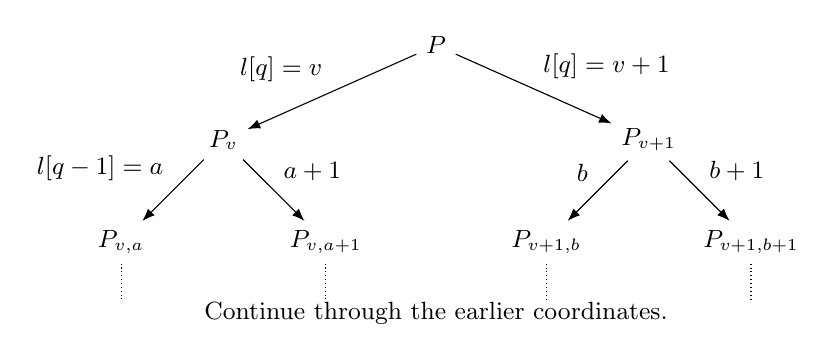
\begin{tikzpicture}[x=1cm,y=1cm,
  every node/.style={font=\small},
  edge/.style={-{Latex[length=1.6mm]},thin}]
\node (root) at (0,0) {$P$};
\node (left) at (-2.7,-1.2) {$P_v$};
\node (right) at (2.7,-1.2) {$P_{v+1}$};
\draw[edge] (root) -- node[above left] {$l[q]=v$} (left);
\draw[edge] (root) -- node[above right] {$l[q]=v+1$} (right);
\node (la) at (-4,-2.5) {$P_{v,a}$};
\node (lb) at (-1.4,-2.5) {$P_{v,a+1}$};
\node (ra) at (1.4,-2.5) {$P_{v+1,b}$};
\node (rb) at (4,-2.5) {$P_{v+1,b+1}$};
\draw[edge] (left) -- node[above left] {$l[q-1]=a$} (la);
\draw[edge] (left) -- node[above right] {$a+1$} (lb);
\draw[edge] (right) -- node[above left] {$b$} (ra);
\draw[edge] (right) -- node[above right] {$b+1$} (rb);
\foreach \name in {la,lb,ra,rb}
  \draw[densely dotted] (\name.south) -- ++(0,-0.45);
\node at (0,-3.4) {Continue through the earlier coordinates.};
\end{tikzpicture}

\caption{The suffix rule used by the shear induction. The bases $a$ and
$b$ may differ because the later coordinate has already been fixed.
Only the separation of siblings is prescribed. Removing leaves, or an
entire subtree, preserves the rule.}
\label{fig:suffix-tree}
\end{figure}

\subsection{Removing a small hole}

The next argument is the classical completion-by-dilation method of
Rogers~\cite{Rog59}. We use the small-dilation form also given by
Fejes T\'oth~\cite[Lemma~2]{FT09}, and include its proof for the
single-lattice setting.

\begin{lemma}[Completion]\label{lem:completion}
Let $K\subset\R^n$ be a convex body and $\Gamma$ a full-rank lattice.
If its hole proportion $\delta=1-|\pi_\Gamma(K)|$ satisfies
\[
 \delta<(1-\delta)k^{-n}
\]
for a positive integer $k$, then $(1+1/k)K+\Gamma=\R^n$.
\end{lemma}

\begin{proof}
Multiplication by $k$ on $\R^n/\Gamma$ maps $\pi_\Gamma(K/k)$
onto $\pi_\Gamma(K)$. Its image has measure at most $k^n$ times
the measure of the original set: partition a fundamental
parallelepiped into $k^n$ cells on which the map is injective.
Consequently
\[
 |\pi_\Gamma(K/k)|\ge k^{-n}(1-\delta)>\delta.
\]
For every point $x$ of the torus, the sets $\pi_\Gamma(K)$ and
$x-\pi_\Gamma(K/k)$ have measures summing to more than one and
therefore intersect. Thus
$\pi_\Gamma(K)+\pi_\Gamma(K/k)$ is the whole torus.
Finally, convexity gives $K+K/k=(1+1/k)K$. Neither symmetry nor
the inclusion $0\in K$ is required.
\end{proof}

\subsection{Proof of the covering theorem}

\begin{proof}[Proof of Theorem~\ref{thm:main}]
All constants in the vertical construction, including its cutoff $B$,
are fixed first. For sufficiently large $n$, put $s=\log\log n$ and
use Proposition~\ref{prop:vertical} with $b_1=\lceil s^2\rceil$.
Retain its notation $L,M,D,D_v,b_i,h_i$, and set
\[
 R^2=\sum_{i=1}^{r+1}b_i h_i^2,\qquad m=n-D.
\]
Here $D=O(s^2+1)$ and $R$ is bounded by a fixed polynomial in $s$.
After passing to the affine coordinates of Lemma~\ref{lem:sections},
there are at most $(Cm^2)^D$ horizontal bodies $J_a$ such that every
$v$ with $\|v\|\le R$ has a label satisfying
\begin{equation}\label{eq:final-sections}
 J_a\subset K_v,\qquad
 c_{\rm sec}\vol_n(K)\gamma_D(v)
 \le\vol_m(J_a)\le
 C_{\rm sec}\vol_n(K)\gamma_D(v).
\end{equation}

Choose an absolute constant $C_*$ later and put
\begin{equation}\label{eq:target-density}
 \rho=C_*n\log n,\qquad
 D_h=\frac{\vol_n(K)}{\rho D_v},\qquad
 u_a=\frac{\vol_m(J_a)}{D_h}.
\end{equation}
For any vertical target $y$, use its pattern from
Proposition~\ref{prop:vertical} and label each raw point $l$ by a
body contained in the section at $y-Ml$. The residual bound permits
Equation~\eqref{eq:final-sections}. With the chosen horizontal covolume,
the normalized section volume is comparable to the corresponding
normalized Gaussian weight multiplied by $\rho$:
\[
 c_{\rm sec}\rho D_v\gamma_D(y-Ml)
 \le u_{a(l)}\le
 C_{\rm sec}\rho D_v\gamma_D(y-Ml).
\]
Thus the total weight supplies the sum of the horizontal loads, while
the atom bound controls each load separately. These estimates give
\begin{equation}\label{eq:final-loads}
 \sum_l u_{a(l)}\ge c_3\rho,\qquad
 \max_l u_{a(l)}\le U_n:=C\rho\exp(-c b_1^{0.70}),
\end{equation}
where $c_3=c_{\rm sec}\kappa>0$ is absolute.

Three scale comparisons are needed. First,
\begin{equation}\label{eq:load-upper-check}
 \frac{U_n}{m}
 \le C'\exp\bigl(s-c's^{1.4}\bigr)\longrightarrow0.
\end{equation}
Second, every pattern has at most $2^D$ points, so deleting those with
$u_{a(l)}<\sqrt m$ loses at most
\begin{equation}\label{eq:load-discard-check}
 2^D\sqrt m=n^{1/2+o(1)}=o(\rho).
\end{equation}
Third, the logarithm of the number of labels is
$O(D\log m)=o(\sqrt m)$. These statements follow from
$D=O(s^2+1)$ and $\log n=e^s$; all their constants are independent
of $K$. In particular the retained pattern is nonempty and has load
at least $c_3\rho/2$ for large $n$.

Restrict the label list to $\sqrt m\le u_a\le U_n$.
Lemma~\ref{lem:horizontal} gives one lattice $\Lambda_h$ of covolume
$D_h$ for which the hole sets
\[
 U_a=(\R^m/\Lambda_h)\setminus\pi_{\Lambda_h}(J_a)
\]
satisfy $|U_a|\le e^{-u_a/2}$ simultaneously. We next select one
shear that works for every retained pattern, not a separate shear
for each target.

\paragraph{A finite family for all targets.}
Initially restrict to $y=Mz$ with $z\in[0,1)^D$. This is enough
because $L$ contains $\Z^D$; after the final lattice is defined,
integer raw translations will reduce any target to this region.
The finite-alphabet conclusion of Proposition~\ref{prop:vertical}
places each scalar raw coordinate in $[-Q_{\rm raw},Q_{\rm raw}]$, where
$Q_{\rm raw}=1+(D+2)^D$. In block $i\le r$ it is a multiple of $1/p_i$;
in the terminal block it is an integer. The logarithmic alphabet size
is therefore at most
\[
 O(D\log(D+2)+\max_i\log p_i)=O(s^{c_0})
\]
for some fixed absolute exponent $c_0$.

Order scalar coordinates by increasing block index, and take
$\mathcal P_q$ to be \emph{all} labeled patterns on the first $q$
coordinate alphabets that are binary by suffixes, for $0\le q\le D$.
This includes every retained full pattern: the base in a block depends
only on later blocks, and deleting points cannot introduce a third
value at any suffix. The families are closed under slicing.

Let $\mathcal A_j$ be the alphabet of scalar coordinate $j$, and let
$N_{\rm lab}$ be the number of retained section labels. A labeled point
consists of a coordinate tuple and one such label, so
$N=N_{\rm lab}\prod_{j=1}^D|\mathcal A_j|$ bounds their number in
each of these coordinate spaces. Consequently
\[
 \log(N+1)=O(D\log n+s^{c_1}),\qquad
 Q:=\sum_{q=0}^D|\mathcal P_q|
       \le (D+1)(N+1)^{2^D}.
\]
For example, the last bound follows by encoding a set of at most
$2^D$ points as a list of that length, padded with a dummy symbol.
Take $L_*=2(Q+1)$. Then
\begin{equation}\label{eq:pattern-cost}
 2^D\log L_*
 \le C4^D(D\log n+s^{c_1})+C2^D\log(D+2)
 =o(n\log n).
\end{equation}
Indeed $4^D$ times any fixed polynomial in $s$ is
$\exp(O(s^2))=o(n)$.

\paragraph{The covering lattice.}
Apply Lemma~\ref{lem:shear} with $\eta_a=e^{-u_a/2}$ and set
$Zl=\sum_{j=1}^D l[j]Z_j$. Define
\begin{equation}\label{eq:full-lattice}
 \Gamma=\{(h+Zl,Ml):h\in\Lambda_h,\ l\in L\}.
\end{equation}
It is a full-rank lattice, being the image of the product lattice
$\Lambda_h\times L$ under an invertible block triangular linear
map. Its covolume is exactly $D_hD_v$, so
$\vol_n(K)/\det\Gamma=\rho$.

For a fixed $y$ and a retained labeled pattern, each $J_{a(l)}$
lies in the section $K_{y-Ml}$. The uncovered horizontal points of
$K+\Gamma$, viewed in $\mathcal T=\R^m/\Lambda_h$, therefore lie in
\[
 \bigcap_l\bigl(U_{a(l)}+\pi_{\Lambda_h}(Zl)\bigr).
\]
For $y\in M[0,1)^D$, Lemma~\ref{lem:shear} and the retained load give
the uniform bound
\begin{equation}\label{eq:uniform-holes}
 \text{horizontal hole fraction at }y
 \le\exp\left(2^D\log L_*-\frac{c_3\rho}{4}\right).
\end{equation}
For other $y$, reduce $M^{-1}y$ modulo $\Z^D$ and translate by the
corresponding point $(Zk,Mk)\in\Gamma$. This only translates the
horizontal section on its torus, so the same bound holds.

Let $F_h,F_v$ be fundamental parallelepipeds of $\Lambda_h$ and
$ML$. Their product is a measurable fundamental domain for
$\Gamma$: first reduce the vertical coordinate using a point
$(Zl,Ml)$, and then reduce the horizontal coordinate using
$\Lambda_h$. The union $K+\Gamma$ is closed, since translates of
the compact set $K$ by a lattice are locally finite. Its complement
is therefore measurable, and Fubini integrates
Equation~\eqref{eq:uniform-holes} over $F_v$. No measurable selection
of auxiliary patterns is needed. Equations~\eqref{eq:target-density}
and~\eqref{eq:pattern-cost} yield
\[
 \delta:=1-|\pi_\Gamma(K)|
 \le\exp\left(o(n\log n)-\frac{c_3C_*}{4}n\log n\right)
 \le n^{-2n}
\]
once $C_*$ is a sufficiently large absolute constant and then $n$
is sufficiently large. Since $n^{-2n}<(1-n^{-2n})n^{-n}$ for
$n\ge2$, Lemma~\ref{lem:completion} with $k=n$ gives
$(1+1/n)K+\Gamma=\R^n$. Thus
\[
 \Lambda=(1+1/n)^{-1}\Gamma
\]
is a single covering lattice for $K$, of density
\[
 \frac{\vol_n(K)}{\det\Lambda}
 =(1+1/n)^n\rho\le eC_*n\log n.
\]

\paragraph{Affine invariance and the remaining dimensions.}
Translations of a body do not change the covering property, and
invertible linear maps applied to both body and lattice preserve
density. Hence the affine normalization can be undone.

There remains only a fixed finite set of dimensions. In each such
dimension choose a maximum-volume simplex with vertices in $K$,
which exists by compactness and has positive volume. Put its vertices
at $0,e_1,\ldots,e_n$ by an affine map. Replacing the $j$th nonzero
vertex by any $x\in K$ changes the determinant to $x_j$, so maximality
gives $|x_j|\le1$. Thus
\[
 [0,1/n]^n\subset K\subset[-1,1]^n.
\]
The lattice $n^{-1}\Z^n$ covers by translates of the smaller cube
and therefore of $K$, with density at most $(2n)^n$.
The maximum of $(2n)^n/(n\log n)$ over the remaining finite set
can be absorbed in one absolute constant. This proves the theorem
for every $n\ge2$.
\end{proof}

\begingroup
\small
\raggedright
\pdfbookmark[1]{References}{references}
\begin{thebibliography}{9}

\bibitem{EK}
Ronen Eldan and Bo'az Klartag,
\emph{Pointwise estimates for marginals of convex bodies},
Journal of Functional Analysis \textbf{254} (2008), no.~8, 2275--2293.
\href{https://doi.org/10.1016/j.jfa.2007.08.014}{doi:10.1016/j.jfa.2007.08.014}.
\href{https://arxiv.org/abs/0708.2513v1}{arXiv:0708.2513v1}.

\bibitem{FT09}
G\'abor Fejes T\'oth,
\emph{A note on covering by convex bodies},
Canadian Mathematical Bulletin \textbf{52} (2009), no.~3, 361--365.
\href{https://doi.org/10.4153/CMB-2009-039-x}{doi:10.4153/CMB-2009-039-x}.

\bibitem{LL}
Heng Li and Xizhi Liu,
\emph{Nearly sharp bounds for lattice coverings by convex bodies},
preprint, version~2, 10~August 2026.
\href{https://arxiv.org/abs/2607.28429v2}{arXiv:2607.28429v2}.

\bibitem{LLC}
Heng Li and Xizhi Liu,
\emph{Two-stage binary correction for nearly linear lattice coverings},
unpolished manuscript, 2026.
\href{https://github.com/xliu2022/xliu2022.github.io/blob/4b360838cb034784293bb6ba2128483fcec6e3ce/Unpolished_Manuscripts/Two-Stage\%20Binary\%20Correction\%20for\%20Nearly\%20Linear\%20Lattice\%20Coverings.pdf}{Author-hosted manuscript},
accessed 23~September 2026.

\bibitem{ORW}
Or Ordentlich, Oded Regev, and Barak Weiss,
\emph{New bounds on the density of lattice coverings},
Journal of the American Mathematical Society \textbf{35} (2022), no.~1,
295--308.
\href{https://doi.org/10.1090/jams/984}{doi:10.1090/jams/984}.
\href{https://arxiv.org/abs/2006.00340v1}{arXiv:2006.00340v1}.

\bibitem{Rog57}
C.~A. Rogers,
\emph{A note on coverings},
Mathematika \textbf{4} (1957), no.~1, 1--6.
\href{https://doi.org/10.1112/S0025579300001030}{doi:10.1112/S0025579300001030}.


\bibitem{Rog58}
C.~A. Rogers,
\emph{Lattice coverings of space: The Minkowski--Hlawka theorem},
Proceedings of the London Mathematical Society (3) \textbf{8} (1958),
447--465.
\href{https://doi.org/10.1112/plms/s3-8.3.447}{doi:10.1112/plms/s3-8.3.447}.

\bibitem{Rog59}
C.~A. Rogers,
\emph{Lattice coverings of space},
Mathematika \textbf{6} (1959), no.~1, 33--39.
\href{https://doi.org/10.1112/S002557930000190X}{doi:10.1112/S002557930000190X}.

\bibitem{Sch58}
Wolfgang M. Schmidt,
\emph{The measure of the set of admissible lattices},
Proceedings of the American Mathematical Society \textbf{9} (1958),
390--403.
\href{https://doi.org/10.2307/2032994}{doi:10.2307/2032994}.
\end{thebibliography}
\endgroup

\end{document}
